\documentclass[titlepage]{article}


\usepackage[margin=1.5in]{geometry}
\usepackage{amsmath}
\usepackage{amsfonts}
\usepackage{booktabs}
\usepackage{pgfplots}
\usepackage{enumitem}
\usepackage{placeins}
\usepackage{graphicx}
\usepackage{subcaption}
\usepackage{fancyvrb}
\usetikzlibrary{matrix,chains,positioning,decorations.pathreplacing,arrows}



\author{Eddie Shim}
\title{Coursera Machine Learning Notes}




\begin{document}
	\maketitle
	
	\section{Regression}
	\subsection{Linear Regression}
	For a univariate linear regression, take a dataset of two variables and optimize the linear equation $y = \theta_1 x + \theta_0$. Use the least squares method $\sum_{i=1}^{m} (f(x) - y)^2$ , where $(f(x)) -y)^2$ represents the residual squared. To minimize residual squared, find $\vec\theta$ which makes the derivative of the cost function equal to 0. 
	
\begin{itemize}
	
	
	\item \textbf{Cost function for linear regression} (where $\vec{\theta} \in \mathbb{R}^{n+1}$, where n is the number of independent variables):
	\begin{align*}
	J(\vec\theta) = \frac{1}{2m} \sum_{i=1}^{m}(h_{\theta}(x^{(i)}) - y^{(i)})^2
	\end{align*}
	
	
	\item \textbf{Gradient descent} (Note: must update all $\theta _j$ simultaneously):
	\begin{align*}
	\theta _j := \theta _j - \alpha \frac{\partial}{\partial \theta _j} J(\vec\theta) 
	\end{align*}
	ex: for 2 variable case: 
	
\begin{align*}
\theta_0 &:= \theta _0 - \alpha \frac{1}{m}\sum_{i=1}^{m} (h_\theta(x^{(i)}) - y^{(i)}) \\
\theta _1 &:= \theta _1 - \alpha \frac{1}{m} \sum_{i=1}^{m} (h_\theta (x^{(i)}) - y^{(i)}) x^{(i)} \\
\end{align*}
	

\item \textbf{Feature scaling}: normalizing all independent variables to an appropriate range. Purpose is to speed up gradient descent.
\begin{align*}
x_i = \frac{x_i - \mu}{\textrm{range of } x}
\end{align*}


\item Note: if $\alpha$ is too large, gradient descent may skip minimum point. However, if $\alpha$ is too little, it may take too long to converge.

\item \textbf{Normal equation} an alternative to gradient descent: 
\begin{align*}
\theta = (X^TX)^{-1}y
\end{align*}

\FloatBarrier
\begin{table} [!htbp]
	\centering
	\begin{tabular}{p{5cm}|p{6cm}}
		\textbf{Gradient Descent} & \textbf{Normal Equation}\\
		\hline
		- need to choose an $\alpha$ & - no need for $\alpha$\\
		- needs many iterations & - no need to iterate, one calculation\\
		- works well even when n is large & - need to compute $(X^TX)^{-1}$ which runs in $O(n^3)$ runtime\\
		& - slow if n is very large
	\end{tabular}
	
	\caption{Pros and Cons}
\end{table}


\newpage

\item \textbf{Vectorization}: to speed up loops.\\
e.g. Transform the following code from: 

\begin{Verbatim}[obeytabs]
for i = 1:3
   for j = 1:m
      theta(i) := theta(i) - alpha * (1/m)*(h_theta(x(j))-y(j))*x(i);
   end
end
\end{Verbatim}


into:
\begin{verbatim}
theta = theta - alpha * delta;
\end{verbatim}

where $\theta \in \mathbb{R}^{n+1},\ \alpha \in \mathbb{R},\ \delta \in \mathbb{R}^{n+1}$

\subsection{Logistic Regression}
\item A classification algorithm (not really regression, which predicts continuous variable given continuous variable)
\begin{align*}
h_\theta (x) &= g(\theta^Tx), \\
\text{where} \ g(z) &= \frac{1}{1+e^{-z}} \ \ \ (\text{sigmoid function})
\end{align*}

\begin{center}
\begin{tikzpicture}
\begin{axis}[xmin = -4, xmax = 4, ymin = 0, ymax=1, xlabel=$z$,ylabel=$g(z)$]
\addplot[very thick, orange] {1/(1+exp{-x})};
\end{axis}
\end{tikzpicture}	
\end{center}

\item Nice properties:
\begin{itemize} [label = $\bullet$]
	\item {$0 \leq h_\theta (x) \leq 1$}, good for properties of a probability
	\item At $z=0$, $g(z) = 0.5$
	\item Converges to $g(z) =1$ quickly as $g$ increases, and vice versa for 0
	\item We can use these properties to output the probability that an input exists in one of two binary states (1 or 0)
\end{itemize}


\item Terminology: the probability of the output of results equaling 1:
\begin{align*}
h_\theta (x) = p(y=1 | \ x;\theta)
\end{align*}


\item Predict $y=1$ if $\theta^T x \geq 0 \Leftrightarrow \text{if} \ h_\theta(x) = g(\theta^Tx) \geq 0.5$

\item Cost Function:
\begin{align*}
J(\vec\theta) = \frac{1}{m} \sum_{i=1}^{m} \text{cost}(h_\theta (x),y)\\
\end{align*}
where cost $(h_\theta(x),y)$ = 
\[ \begin{cases} 
-log(h_\theta(x)) \ &\text{if} \  y=1\\ 
-log(1-h_\theta(x)) \ &\text{if} \  y =0 
\end{cases} \]


\begin{figure}[h]
	\begin{minipage}{.55\textwidth}
			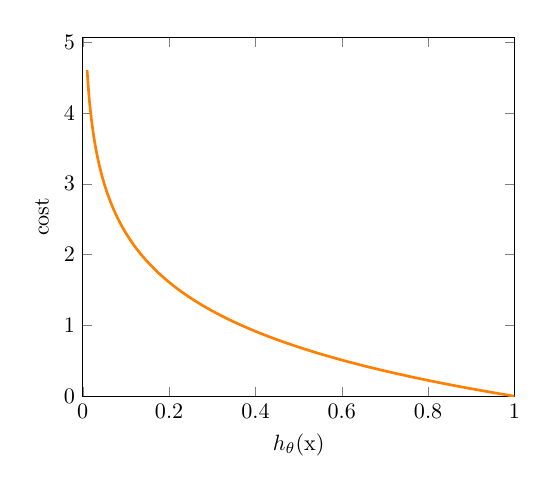
\begin{tikzpicture}[scale=0.8]
			\begin{axis}[xmin=0,xmax=1,ymin=0,xlabel=$h_\theta$(x),ylabel=cost]
			\addplot[very thick,orange, domain=0.01:4.5,smooth,samples=1000] {-ln(x)};
			\end{axis}
			\end{tikzpicture}	
			
	\end{minipage}
		\begin{minipage}{.01\textwidth}
			
			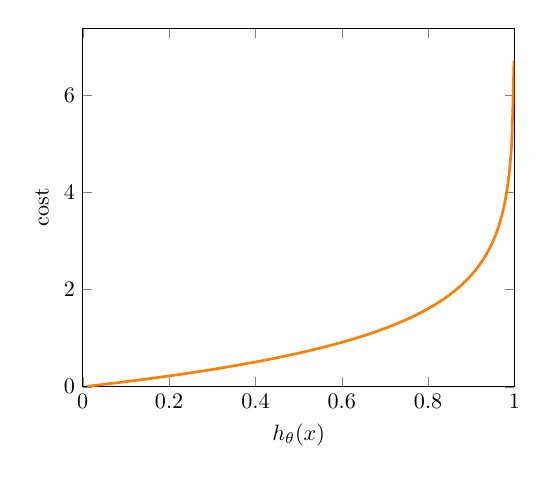
\begin{tikzpicture}[scale=0.8]
			\begin{axis}[xmin=0, xmax=1,xlabel=$h_\theta(x)$,ylabel=cost, ymin=0]
			\addplot[very thick,orange, domain=0.01:4.5,smooth,samples=1000] {-ln(1-x)};
			\end{axis}
			\end{tikzpicture}
			
		\end{minipage}	
		
		\caption{Left: $-log(h_\theta (x))$ ; Right: $-log(1-h_\theta (x))$}
	
	
\end{figure}

\item We can create a more succinct function instead of using a piecewise function.\\
\textbf{Cost function for logistic regression}:

\begin{align*} 
\text{cost}(h_\theta(x),y) &= -y*log(h_\theta(x)) - (1-y)*log(1-h_\theta(x))\\
J(\vec{\theta}) &= -\frac{1}{m}\Big(\sum_{i=1}^{m} y^{(i)}*log(h_\theta(x^{(i)})) + (1-y^{(i)})*log(1-h_\theta(x^{(i)}))\Big)
\end{align*}


\subsection{Neural Networks}

\def\layersep{2.5cm}
\begin{tikzpicture}[shorten >=1pt,->,draw=black!50, node distance=\layersep]
\tikzstyle{every pin edge}=[<-,shorten <=1pt]
\tikzstyle{neuron}=[circle,fill=black!25,minimum size=17pt,inner sep=0pt]
\tikzstyle{input neuron}=[neuron, fill=green!50];
\tikzstyle{output neuron}=[neuron, fill=red!50];
\tikzstyle{hidden neuron}=[neuron, fill=blue!50];
\tikzstyle{annot} = [text width=4em, text centered]

% Draw the input layer nodes
\foreach \name / \y in {1,...,4}
% This is the same as writing \foreach \name / \y in {1/1,2/2,3/3,4/4}
\node[input neuron, pin=left:Input \#\y] (I-\name) at (0,-\y) {};

% Draw the hidden layer nodes
\foreach \name / \y in {1,...,5}
\path[yshift=0.5cm]
node[hidden neuron] (H-\name) at (\layersep,-\y cm) {};

% Draw the output layer node
\node[output neuron,pin={[pin edge={->}]right:Output}, right of=H-3] (O) {};

% Connect every node in the input layer with every node in the
% hidden layer.
\foreach \source in {1,...,4}
\foreach \dest in {1,...,5}
\path (I-\source) edge (H-\dest);

% Connect every node in the hidden layer with the output layer
\foreach \source in {1,...,5}
\path (H-\source) edge (O);

% Annotate the layers
\node[annot,above of=H-1, node distance=1cm] (hl) {Hidden layer};
\node[annot,left of=hl] {Input layer};
\node[annot,right of=hl] {Output layer};
\end{tikzpicture}

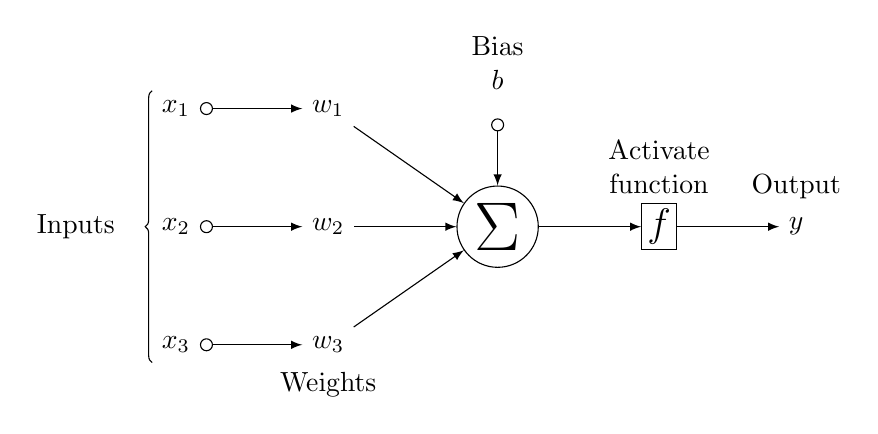
\begin{tikzpicture}[
init/.style={
	draw,
	circle,
	inner sep=2pt,
	font=\Huge,
	join = by -latex
},
squa/.style={
	draw,
	inner sep=2pt,
	font=\Large,
	join = by -latex
},
start chain=2,node distance=13mm
]
\node[on chain=2] 
(x2) {$x_2$};
\node[on chain=2,join=by o-latex] 
{$w_2$};
\node[on chain=2,init] (sigma) 
{$\displaystyle\Sigma$};
\node[on chain=2,squa,label=above:{\parbox{2cm}{\centering Activate \\ function}}]   
{$f$};
\node[on chain=2,label=above:Output,join=by -latex] 
{$y$};
\begin{scope}[start chain=1]
\node[on chain=1] at (0,1.5cm) 
(x1) {$x_1$};
\node[on chain=1,join=by o-latex] 
(w1) {$w_1$};
\end{scope}
\begin{scope}[start chain=3]
\node[on chain=3] at (0,-1.5cm) 
(x3) {$x_3$};
\node[on chain=3,label=below:Weights,join=by o-latex] 
(w3) {$w_3$};
\end{scope}
\node[label=above:\parbox{2cm}{\centering Bias \\ $b$}] at (sigma|-w1) (b) {};

\draw[-latex] (w1) -- (sigma);
\draw[-latex] (w3) -- (sigma);
\draw[o-latex] (b) -- (sigma);

\draw[decorate,decoration={brace,mirror}] (x1.north west) -- node[left=10pt] {Inputs} (x3.south west);
\end{tikzpicture}


\end{itemize}
\end{document}
